% Компиляция: pdfLaTeX -> BibTeX -> pdfLaTeX -> pdfLaTeX
% fontenc загружается до beamer, иначе hyperref теряет кириллицу в закладках PDF
\RequirePackage[T2A]{fontenc}
\documentclass[t,aspectratio=169,11pt,hyperref={unicode}]{beamer}

\usepackage{cmap}
\usepackage[utf8]{inputenc}
\usepackage[english,russian]{babel}
\usepackage[numbers,sort&compress]{natbib}
\usepackage{amsmath,amssymb}
\usepackage{booktabs}
\usepackage{tabularx}
\usepackage{appendixnumberbeamer}

%======================================================================
% Оформление: белый фон, один тёмно-синий цвет, без значков и теней
%======================================================================
\usetheme{default}
\usefonttheme[onlymath]{serif}
\setbeamertemplate{navigation symbols}{}
\setbeamersize{text margin left=1cm,text margin right=1cm}

\definecolor{accent}{HTML}{1B365D}
\definecolor{muted}{HTML}{6B6B6B}
\definecolor{hairline}{HTML}{B4B4B4}

\setbeamercolor{normal text}{fg=black}
\setbeamercolor{structure}{fg=accent}
\setbeamercolor{frametitle}{fg=accent}
\setbeamercolor{title}{fg=accent}
\setbeamercolor{footline}{fg=muted}
\setbeamercolor{block title}{fg=accent,bg=}
\setbeamercolor{block body}{fg=black,bg=}

\setbeamerfont{frametitle}{size=\large,series=\bfseries}
\setbeamerfont{title}{size=\Large,series=\bfseries}
\setbeamerfont{author}{size=\normalsize}
\setbeamerfont{date}{size=\normalsize}
\setbeamerfont{institute}{size=\small}
\setbeamerfont{footline}{size=\scriptsize}
\setbeamerfont{block title}{size=\normalsize,series=\bfseries}

% Списки: тире и «1)»
\setbeamertemplate{itemize item}{\textendash}
\setbeamertemplate{itemize subitem}{\textendash}
\setbeamertemplate{enumerate item}{\insertenumlabel)}
\setbeamertemplate{blocks}[default]

\makeatletter
% Заголовок слайда с тонкой линией под ним
\newlength{\innerw}
\setbeamertemplate{frametitle}{%
  \setlength{\innerw}{\dimexpr\paperwidth-\beamer@leftmargin-\beamer@rightmargin\relax}%
  \nointerlineskip
  \vskip1.6ex
  \vbox{\hsize=\innerw\raggedright
    \usebeamerfont{frametitle}\usebeamercolor[fg]{frametitle}\insertframetitle\par}%
  \vskip0.9ex
  \hbox{\textcolor{accent}{\rule{\innerw}{0.6pt}}}%
  \vskip-0.8ex
}

% Подвал: автор | краткое название | номер слайда
\newcommand{\footnumber}{\insertframenumber\,/\,\inserttotalframenumber}
\setbeamertemplate{footline}{%
  \setlength{\innerw}{\dimexpr\paperwidth-\beamer@leftmargin-\beamer@rightmargin\relax}%
  \hbox to\paperwidth{\hskip\beamer@leftmargin
    \textcolor{hairline}{\rule{\innerw}{0.4pt}}\hss}%
  \vskip0.7ex
  \hbox to\paperwidth{\hskip\beamer@leftmargin
    \usebeamerfont{footline}\usebeamercolor[fg]{footline}%
    \makebox[0.25\innerw][l]{\insertshortauthor}\hfill
    \makebox[0.5\innerw][c]{\insertshorttitle}\hfill
    \makebox[0.25\innerw][r]{\footnumber}%
    \hskip\beamer@rightmargin}%
  \vskip1.5ex
}

% Титульный слайд
\setbeamertemplate{title page}{%
  \vfill
  \centering
  {\usebeamerfont{institute}\usebeamercolor[fg]{footline}\insertinstitute\par}
  \vskip2em
  {\usebeamerfont{title}\usebeamercolor[fg]{title}\inserttitle\par}
  \vskip1.2em
  {\color{accent}\rule{0.3\textwidth}{0.6pt}\par}
  \vskip1.2em
  {\usebeamerfont{author}\insertauthor\par}
  \vskip0.5em
  {\usebeamerfont{date}\usebeamercolor[fg]{footline}\insertdate\par}
  \vfill
}
\makeatother

% Список литературы: номера [1], [2], ... без значков
\setbeamertemplate{frametitle continuation}{}
\setbeamertemplate{bibliography item}[text]
\setbeamertemplate{bibliography entry article}{}
\setbeamertemplate{bibliography entry title}{}
\setbeamertemplate{bibliography entry location}{}
\setbeamertemplate{bibliography entry note}{}
\setbeamercolor*{bibliography item}{fg=black}
\setbeamercolor*{bibliography entry author}{fg=black}
\setbeamercolor*{bibliography entry title}{fg=black}
\setbeamercolor*{bibliography entry location}{fg=black}
\setbeamercolor*{bibliography entry note}{fg=black}

\newcolumntype{L}{>{\raggedright\arraybackslash}X}

\title[Сходимость представлений нейросетей]{Сходимость представлений нейросетей
  разных архитектур, модальностей и~задач на~примере рекомендательных систем}
\author[Талменев В.\,А.]{Талменев Владимир Александрович}
\institute{Центральный университет\\Научный трек}
\date{11 ноября 2026~г.}

\begin{document}

% Нумерация источников совпадает с порядком в списке литературы
\nocite{huh2024platonic,koepke2026cave,groger2026aristotelian,jha2025vec2vec,
  balestriero2026jepa,maniparambil2024,sharma2024checkup,merullo2023linearly,
  moschella2023relative,bansal2021stitching,dravid2023rosetta,ainsworth2023rebasin,
  abdou2021color,kornblith2019cka,klabunde2025survey,davari2023cka,
  sucholutsky2023aligned,kang2018sasrec,sun2019bert4rec,xie2022cl4srec,
  hou2022unisrec,li2023recformer,yuan2023idvsmodality,sheng2025alpharec,
  collins2025complementarity,zhang2023collm,liao2024llara,zhai2024hstu,
  rajput2023tiger,lin2024dreamumm,iana2024peeling,oord2018cpc,levy2014implicit,
  barkan2016item2vec,radford2021clip,oquab2024dinov2,lenc2015equivariance}

\begin{frame}[plain,noframenumbering,c]
\titlepage
\end{frame}

%----------------------------------------------------------------------
\begin{frame}{Тема и цель исследования}
Исследуется сходимость представлений нейросетей разных архитектур, модальностей
и~задач на~примере рекомендательных систем.

\medskip
Основа~--- гипотеза платоновского представления~\cite{huh2024platonic}: с~ростом
масштаба модели разных архитектур и~модальностей сходятся к~общей статистической
модели реальности. Гипотеза
\begin{itemize}
  \item проверена только для зрения и~текста~\cite{huh2024platonic,maniparambil2024};
  \item зависит от размера выборки и~калибровки мер
    сходства~\cite{koepke2026cave,groger2026aristotelian};
  \item для рекомендательных моделей не проверялась.
\end{itemize}

\medskip
\begin{block}{Цель исследования~---}
выяснить, сходятся~ли представления товаров у~рекомендательных моделей между собой
и~с~языковыми моделями и~от каких факторов это зависит.
\end{block}
\end{frame}

%----------------------------------------------------------------------
\begin{frame}{Обзор литературы}
\vspace{0.5em}
\begingroup
\footnotesize
\renewcommand{\arraystretch}{1.04}
\begin{tabularx}{\textwidth}{@{}>{\raggedright\arraybackslash}p{0.33\textwidth}LL@{}}
\toprule
\textbf{Группа работ} & \textbf{Достоинства} & \textbf{Ограничения} \\
\midrule
Склейка и~отображения~\cite{merullo2023linearly,moschella2023relative,bansal2021stitching,dravid2023rosetta}
  & Прямо проверяют совместимость & Нужно обучать отображение \\
Соседи: зрение и~язык~\cite{huh2024platonic,maniparambil2024,sharma2024checkup}
  & Простая мера, растёт с~масштабом & Зависит от выборки и~$k$~\cite{koepke2026cave} \\
Меры и~калибровка~\cite{groger2026aristotelian,kornblith2019cka,klabunde2025survey,davari2023cka}
  & Калибровка убирает завышение~\cite{groger2026aristotelian} & CKA неустойчива~\cite{davari2023cka} \\
Теория~\cite{huh2024platonic,balestriero2026jepa,oord2018cpc,levy2014implicit}
  & Объясняет сходимость к~ядру PMI & Идеализированные допущения \\
Язык в~рекомендациях~\cite{hou2022unisrec,li2023recformer,yuan2023idvsmodality,sheng2025alpharec}
  & Линейное отображение работает~\cite{sheng2025alpharec} & Мерят качество, а~не геометрию \\
Сравнение рекомендателей~\cite{collins2025complementarity,iana2024peeling}
  & ID и~текст дополняют друг друга~\cite{collins2025complementarity} & Нет связи с~гипотезой и~масштабом \\
\bottomrule
\end{tabularx}
\endgroup

\smallskip
\small
Основа работы~--- протокол~\cite{huh2024platonic}, калиброванные
меры~\cite{groger2026aristotelian} и~линейное отображение~\cite{sheng2025alpharec}.
Сходимость рекомендательных моделей с~учётом критики мер не исследовалась.
\end{frame}

%----------------------------------------------------------------------
\begin{frame}{Постановка задачи}
\small
\setlength{\abovedisplayskip}{3pt}\setlength{\belowdisplayskip}{3pt}
Решается задача оценки сходимости представлений товаров у~разных моделей.

\smallskip
Заданы
\begin{enumerate}
  \item товары $\mathcal{I}=\{1,\dots,n\}$, взаимодействия $R\in\{0,1\}^{m\times n}$,
    описания товаров $t_1,\dots,t_n$;
  \item рекомендательная модель $f_\theta\colon\mathcal{I}\to\mathbb{R}^{d}$ и~языковая
    модель $g\colon t_i\mapsto g(t_i)\in\mathbb{R}^{d'}$ с~матрицами представлений
    $F_\theta\in\mathbb{R}^{n\times d}$, $G\in\mathbb{R}^{n\times d'}$.
\end{enumerate}

\smallskip
Внутренний критерий ($\omega$~--- размер модели, объём данных, число задач, $\lambda$):
\[
  \theta^{*}(\omega)=\arg\min_{\theta}\,\mathcal{L}_{\mathrm{rec}}(\theta;R_\omega)
  +\lambda\|\theta\|_2^2.
\]

\smallskip
Сходство пространств~--- калиброванная доля общих $k$ ближайших соседей:
\[
  m_k(F,G)=\frac{1}{nk}\sum\nolimits_{i=1}^{n}\bigl|N_k^F(i)\cap N_k^G(i)\bigr|,\qquad
  \tilde m_k=m_k(F,G)-\mathbb{E}_{\pi}\,m_k(F,G_{\pi}).
\]
Внешний критерий~--- Recall@$K$ и~NDCG@$K$ на отложенном последнем товаре.

\smallskip
Требуется найти зависимость $\tilde m_k\bigl(F_{\theta^{*}(\omega)},G\bigr)$ от~$\omega$
и~от NDCG@$K$; эталон~--- $K_{\mathrm{PMI}}(i,j)=\log\bigl(P(i,j)/P(i)P(j)\bigr)$.
\end{frame}

%----------------------------------------------------------------------
\begin{frame}{Базовый эксперимент: воспроизведение~\cite{huh2024platonic}}
Цель эксперимента~--- проверить меру и~протокол на~данных основной статьи
до перехода к~рекомендательным моделям.

\medskip
\small
\renewcommand{\arraystretch}{1.3}
\begin{tabularx}{\textwidth}{@{}p{0.17\textwidth}L@{}}
\toprule
Данные & WIT-1024: 1024 пары «картинка~--- подпись» из Википедии~\cite{huh2024platonic} \\
Модели & языковые BLOOMZ от 0,56 до 7,1 млрд параметров; модели зрения DINOv2-S, -B, -L, -G \\
Мера & mutual $k$-NN, $k=10$, максимум по парам слоёв; контроль~--- перемешанные пары \\
Ожидание & выше случайного уровня $k/(n-1)\approx0{,}01$ и~рост с~размером
  модели~\cite{huh2024platonic}; для OpenLLaMA-3B и~DINOv2-B получено
  0,135~\cite{koepke2026cave} \\
\bottomrule
\end{tabularx}
\end{frame}

%----------------------------------------------------------------------
\begin{frame}{Результаты базового эксперимента}
\begin{columns}[T,onlytextwidth]
\begin{column}{0.52\textwidth}
\vspace{-2pt}
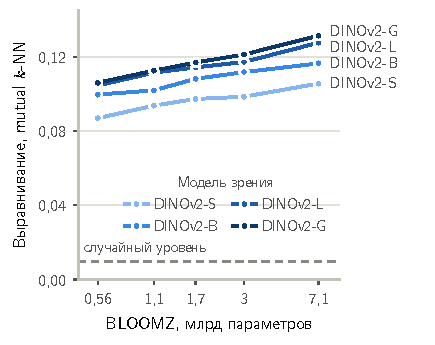
\includegraphics[width=\linewidth]{figures/wit1024_alignment_slides.pdf}
\end{column}
\begin{column}{0.45\textwidth}
\small
\begin{itemize}
  \item выравнивание растёт с~размером обеих моделей: от~0,087 до~0,131;
  \item лучшая пара BLOOMZ-7b1 и~DINOv2-G~--- в~13~раз выше случайного уровня;
  \item на~перемешанных парах~--- 0,0098, то~есть случайный уровень;
  \item лучшие слои~--- в~конце обеих сетей.
\end{itemize}
\end{column}
\end{columns}

\vfill
\small
Порядок величины тот~же, что в~\cite{koepke2026cave}; там~же показано, что на~больших
выборках значение падает. Далее~--- рекомендательные модели на~MovieLens.
\end{frame}

%----------------------------------------------------------------------
\appendix
\setbeamertemplate{footline}{}

\begin{frame}[t,allowframebreaks]{Список литературы}
\scriptsize
\setlength{\bibsep}{1.5pt}
\begin{otherlanguage*}{english}
\bibliographystyle{IEEEtran}
\bibliography{refs}
\end{otherlanguage*}
\end{frame}

\end{document}
